\chapter{Metodologi dan Rancangan}

\section{Penjelasan Metodologi}

Pengerjaan Tugas Akhir yang meliputi pengembangan sistem mengikuti alur yang terdapat pada Gambar \ref{fig:waterfall}. Alur yang digunakan adalah alur \textit{waterfall}. Alur tersebut memungkinkan untuk kembali ke tahap sebelumnya jika pada tahap tertentu terjadi kesalahan. Tahap pertama dalam alur adalah penelitian. Penelitian dilakukan untuk menentukan algoritma yang cocok untuk diterapkan ke dalam sistem. Lalu, tahap kedua adalah perancangan sistem. Perancangan dilakukan untuk menentukan tahap-tahap yang akan dilakukan oleh sistem. Kemudian, tahap selanjutnya adalah pengembangan sistem, yang mana merupakan tahap untuk pengembangan dari rancangan sistem yang telah dibuat sebelumnya. Tahap terakhir pada alur pengembangan adalah pengujian sistem.

\begin{figure}[H]
	\centering
	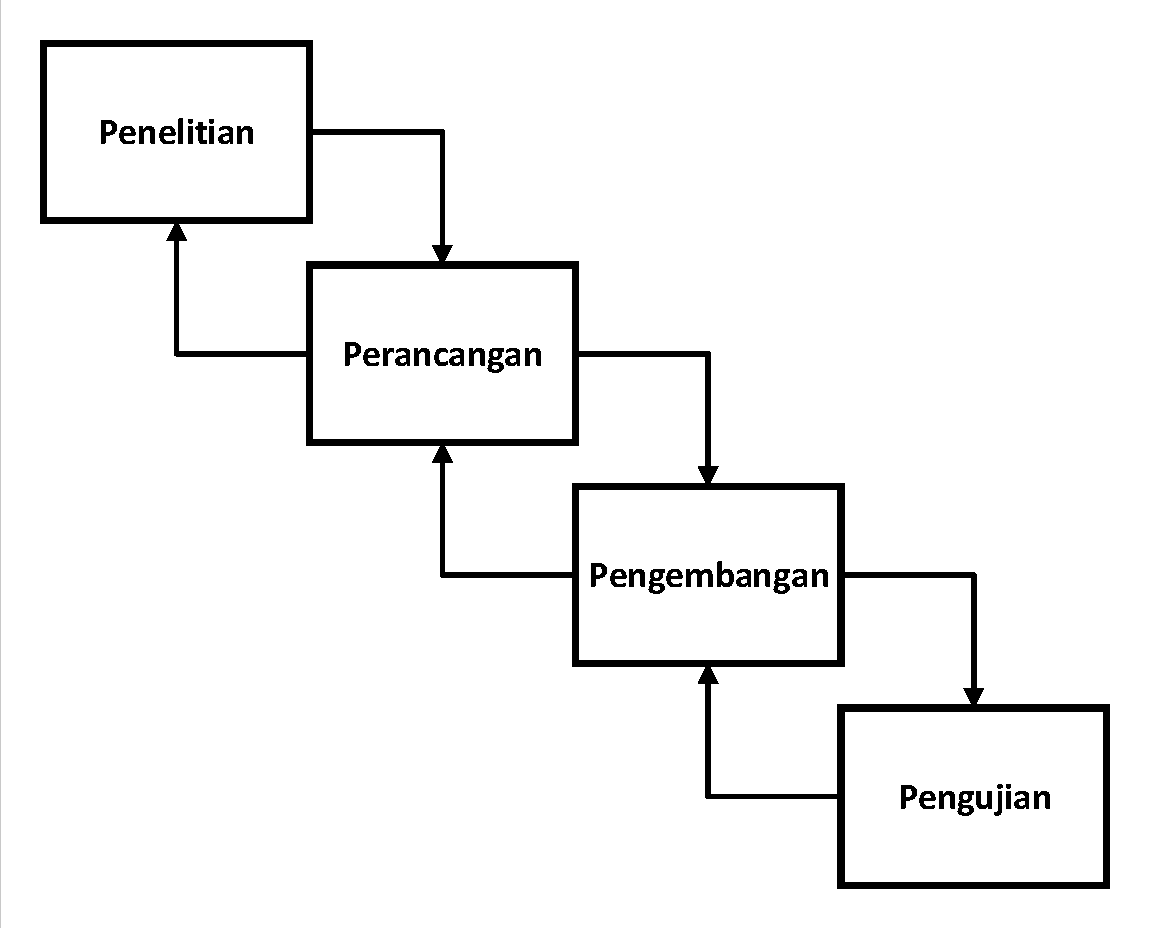
\includegraphics[width=0.7\textwidth, trim=2 2 2 2, clip]{resources/3/waterfall.pdf}
	\caption{Alur \textit{waterfall} untuk pengembangan sistem}
	\label{fig:waterfall}
\end{figure}

\section{Algoritma untuk Pelatihan Pengenalan Entitas}

Teknik yang dilakukan untuk bagian pengenalan entitas adalah teknik \textit{sequence labeling}, seperti yang tertera pada Gambar \ref{fig:sequence_labeling}. Sebuah kalimat yang disediakan oleh data latih menyertakan kata-kata yang merupakan bagian dari entitas. Kalimat tersebut dipecahkan menjadi \textit{token-token}. Tiap \textit{token} berisi sebuah kata dalam kalimat. Tiap \textit{token} ditandai dengan label-label, menandakan apakah \textit{token} tersebut merupakan entitas atau tidak. Susunan \textit{token} dan label tersebut akan menjadi acuan untuk pelatihan pengenalan entitas.

\begin{figure}[H]
	\centering
	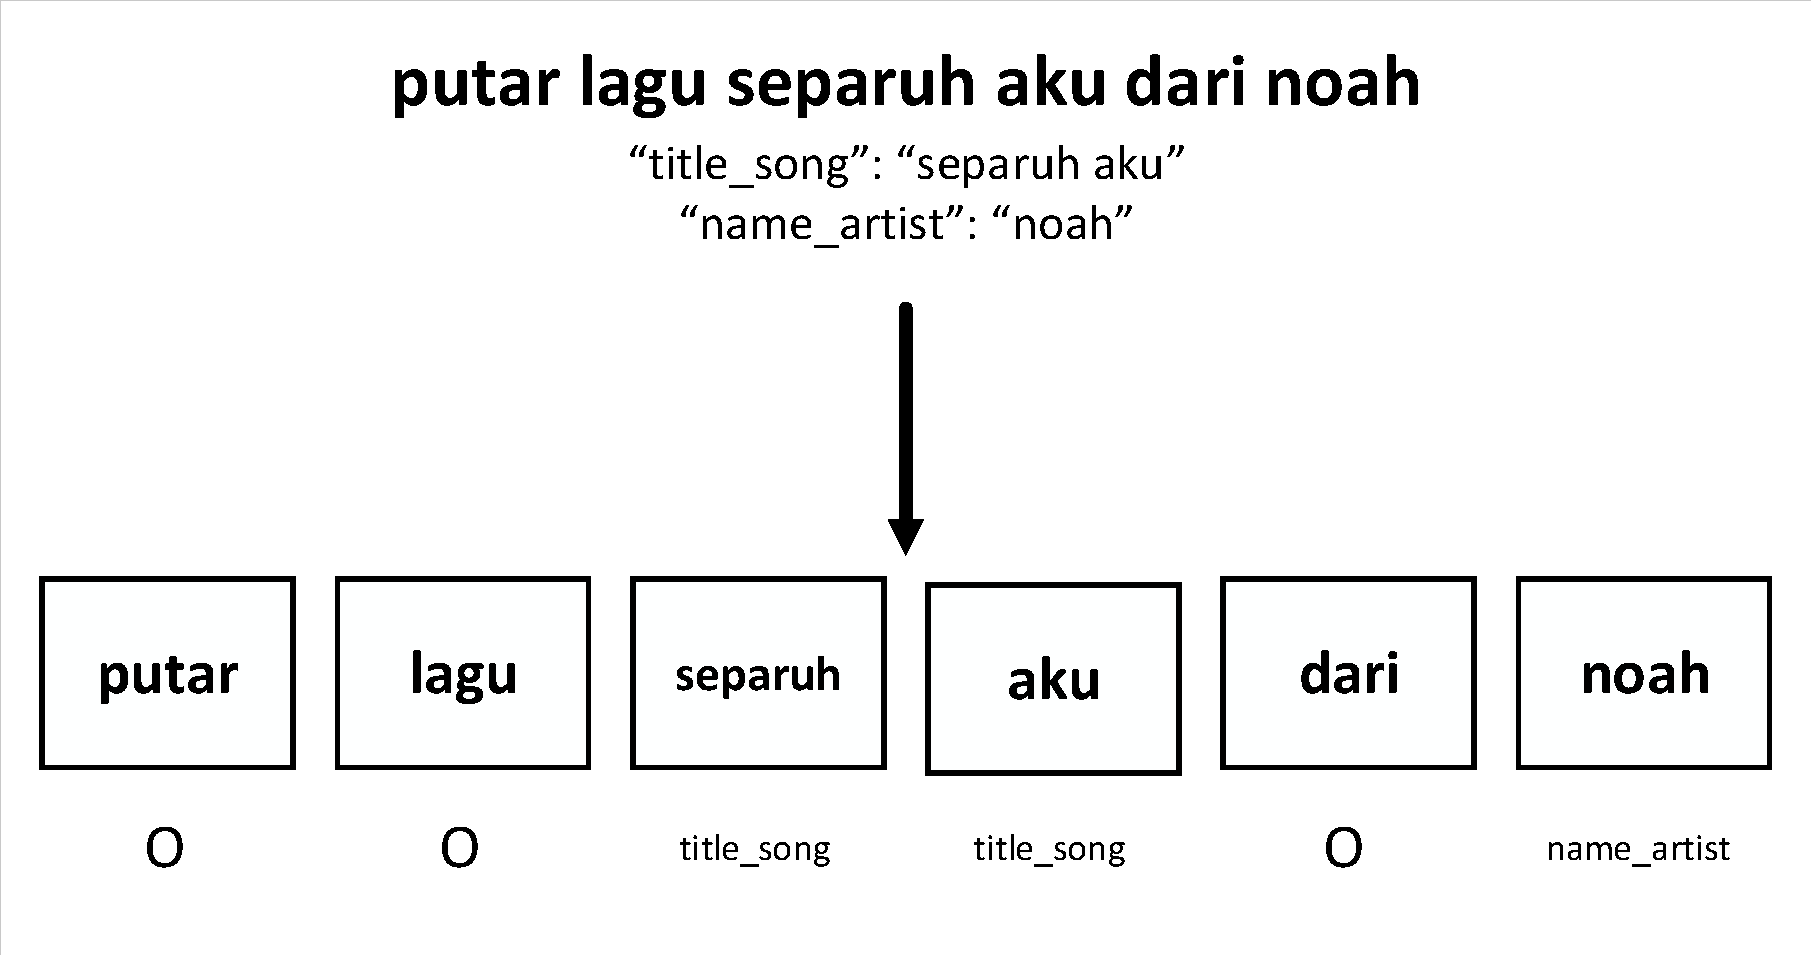
\includegraphics[width=0.9\textwidth, trim=2 2 2 2, clip]{resources/3/sequence_labeling.pdf}
	\caption{Teknik \textit{sequence labeling}}
	\label{fig:sequence_labeling}
\end{figure}

Melihat kelemahan yang terdapat pada pengenalan entitas milik Rasa NLU, beberapa variasi algoritma dapat digunakan untuk mengganti pelatihan pengenalan entitas tersebut.

\subsection{\textit{Convolutional Neural Network} (CNN)}

Gambar \ref{fig:cnn} menunjukkan arsitektur lapisan CNN yang digunakan untuk melakukan latihan pengenalan entitas ini, dibangun dengna menggunakan Keras \parencite{sasank2017spoken}. Lapisan pertama diawali dengan melakukan \textit{embedding} terhadap kumpulan kata dalam sebuah kalimat yang ingin dilatih. Kemudian, hasil \textit{embedding} dimasukkan ke lapisan \textit{convolutional} satu dimensi. Selanjutnya, luaran dari lapisan \textit{convolutional} dikurangi sebesar 0,25 persen pada lapisan \textit{dropout}. Hal ini bertujuan untuk meningkatkan kinerja pembelajaran sebuah model. Setelah itu, luaran yang telah dikurangi dimasukkan ke dalam lapisan \textit{gated recurrent unit} (GRU). Terakhir, luaran GRU dimasukkan ke lapisan \textit{neural network} yang terdistribusi berdasarkan \textit{timestep} dengan menggunakan pembungkus TimeDistributed.

\begin{figure}[H]
	\centering
	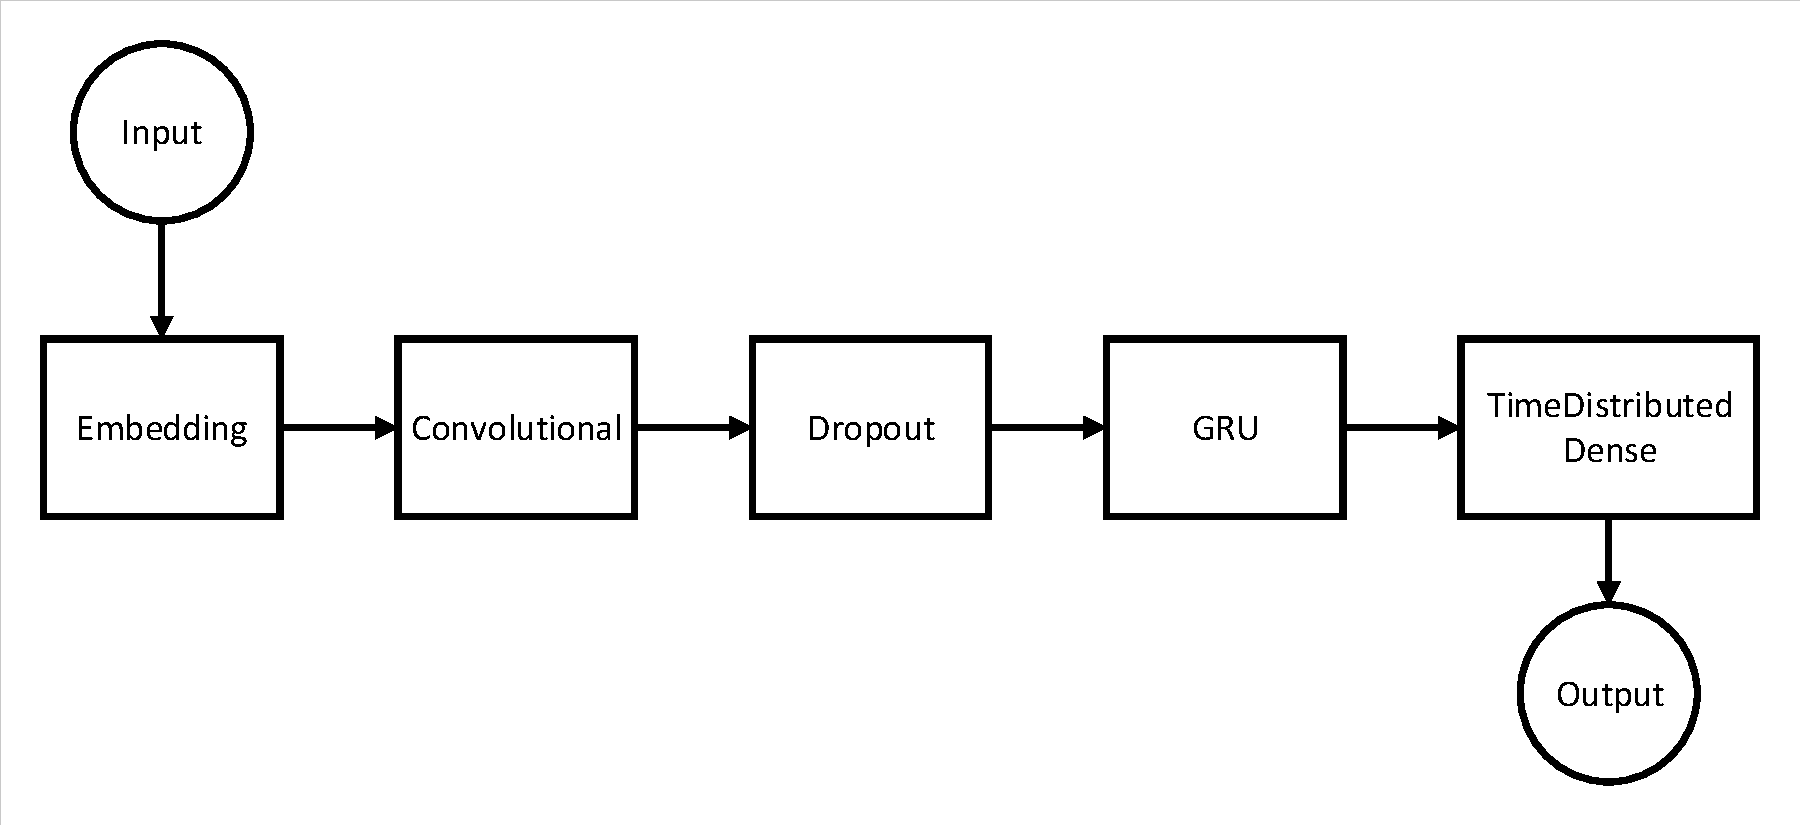
\includegraphics[width=0.9\textwidth, trim=2 2 2 2, clip]{resources/3/cnn.pdf}
	\caption{Arsitektur CNN \parencite{sasank2017spoken}}
	\label{fig:cnn}
\end{figure}

\subsection{LSTM Dua Arah dan CRF}

LSTM dua arah merujuk kepada penggunaan dua LSTM dengan dua arah berlawanan, yaitu maju dan mundur. Hal ini untuk menutup kelemahan LSTM yang hanya melihat pada kata sebelum kata yang sedang dilatih. LSTM pertama dipasang dari awal kalimat dan bergerak maju, sedangkan LSTM kedua dipasang dari akhir kalimat dan bergerak mundur.

Arsitektur yang akan digunakan ditunjukkan pada Gambar \ref{fig:blstmcrf} \parencite{lample2016neural}. Arsitektur ini melibatkan LSTM dua arah. Masukan kedua LSTM didapatkan dari proses \textit{embedding} sebuah kata, tergantung pada urutan luaran \textit{embedding} itu terhadap kedua LSTM. Kedua luaran LSTM tersebut akhirnya disatukan untuk menjadi masukan lapisan CRF.

\begin{figure}[H]
	\centering
	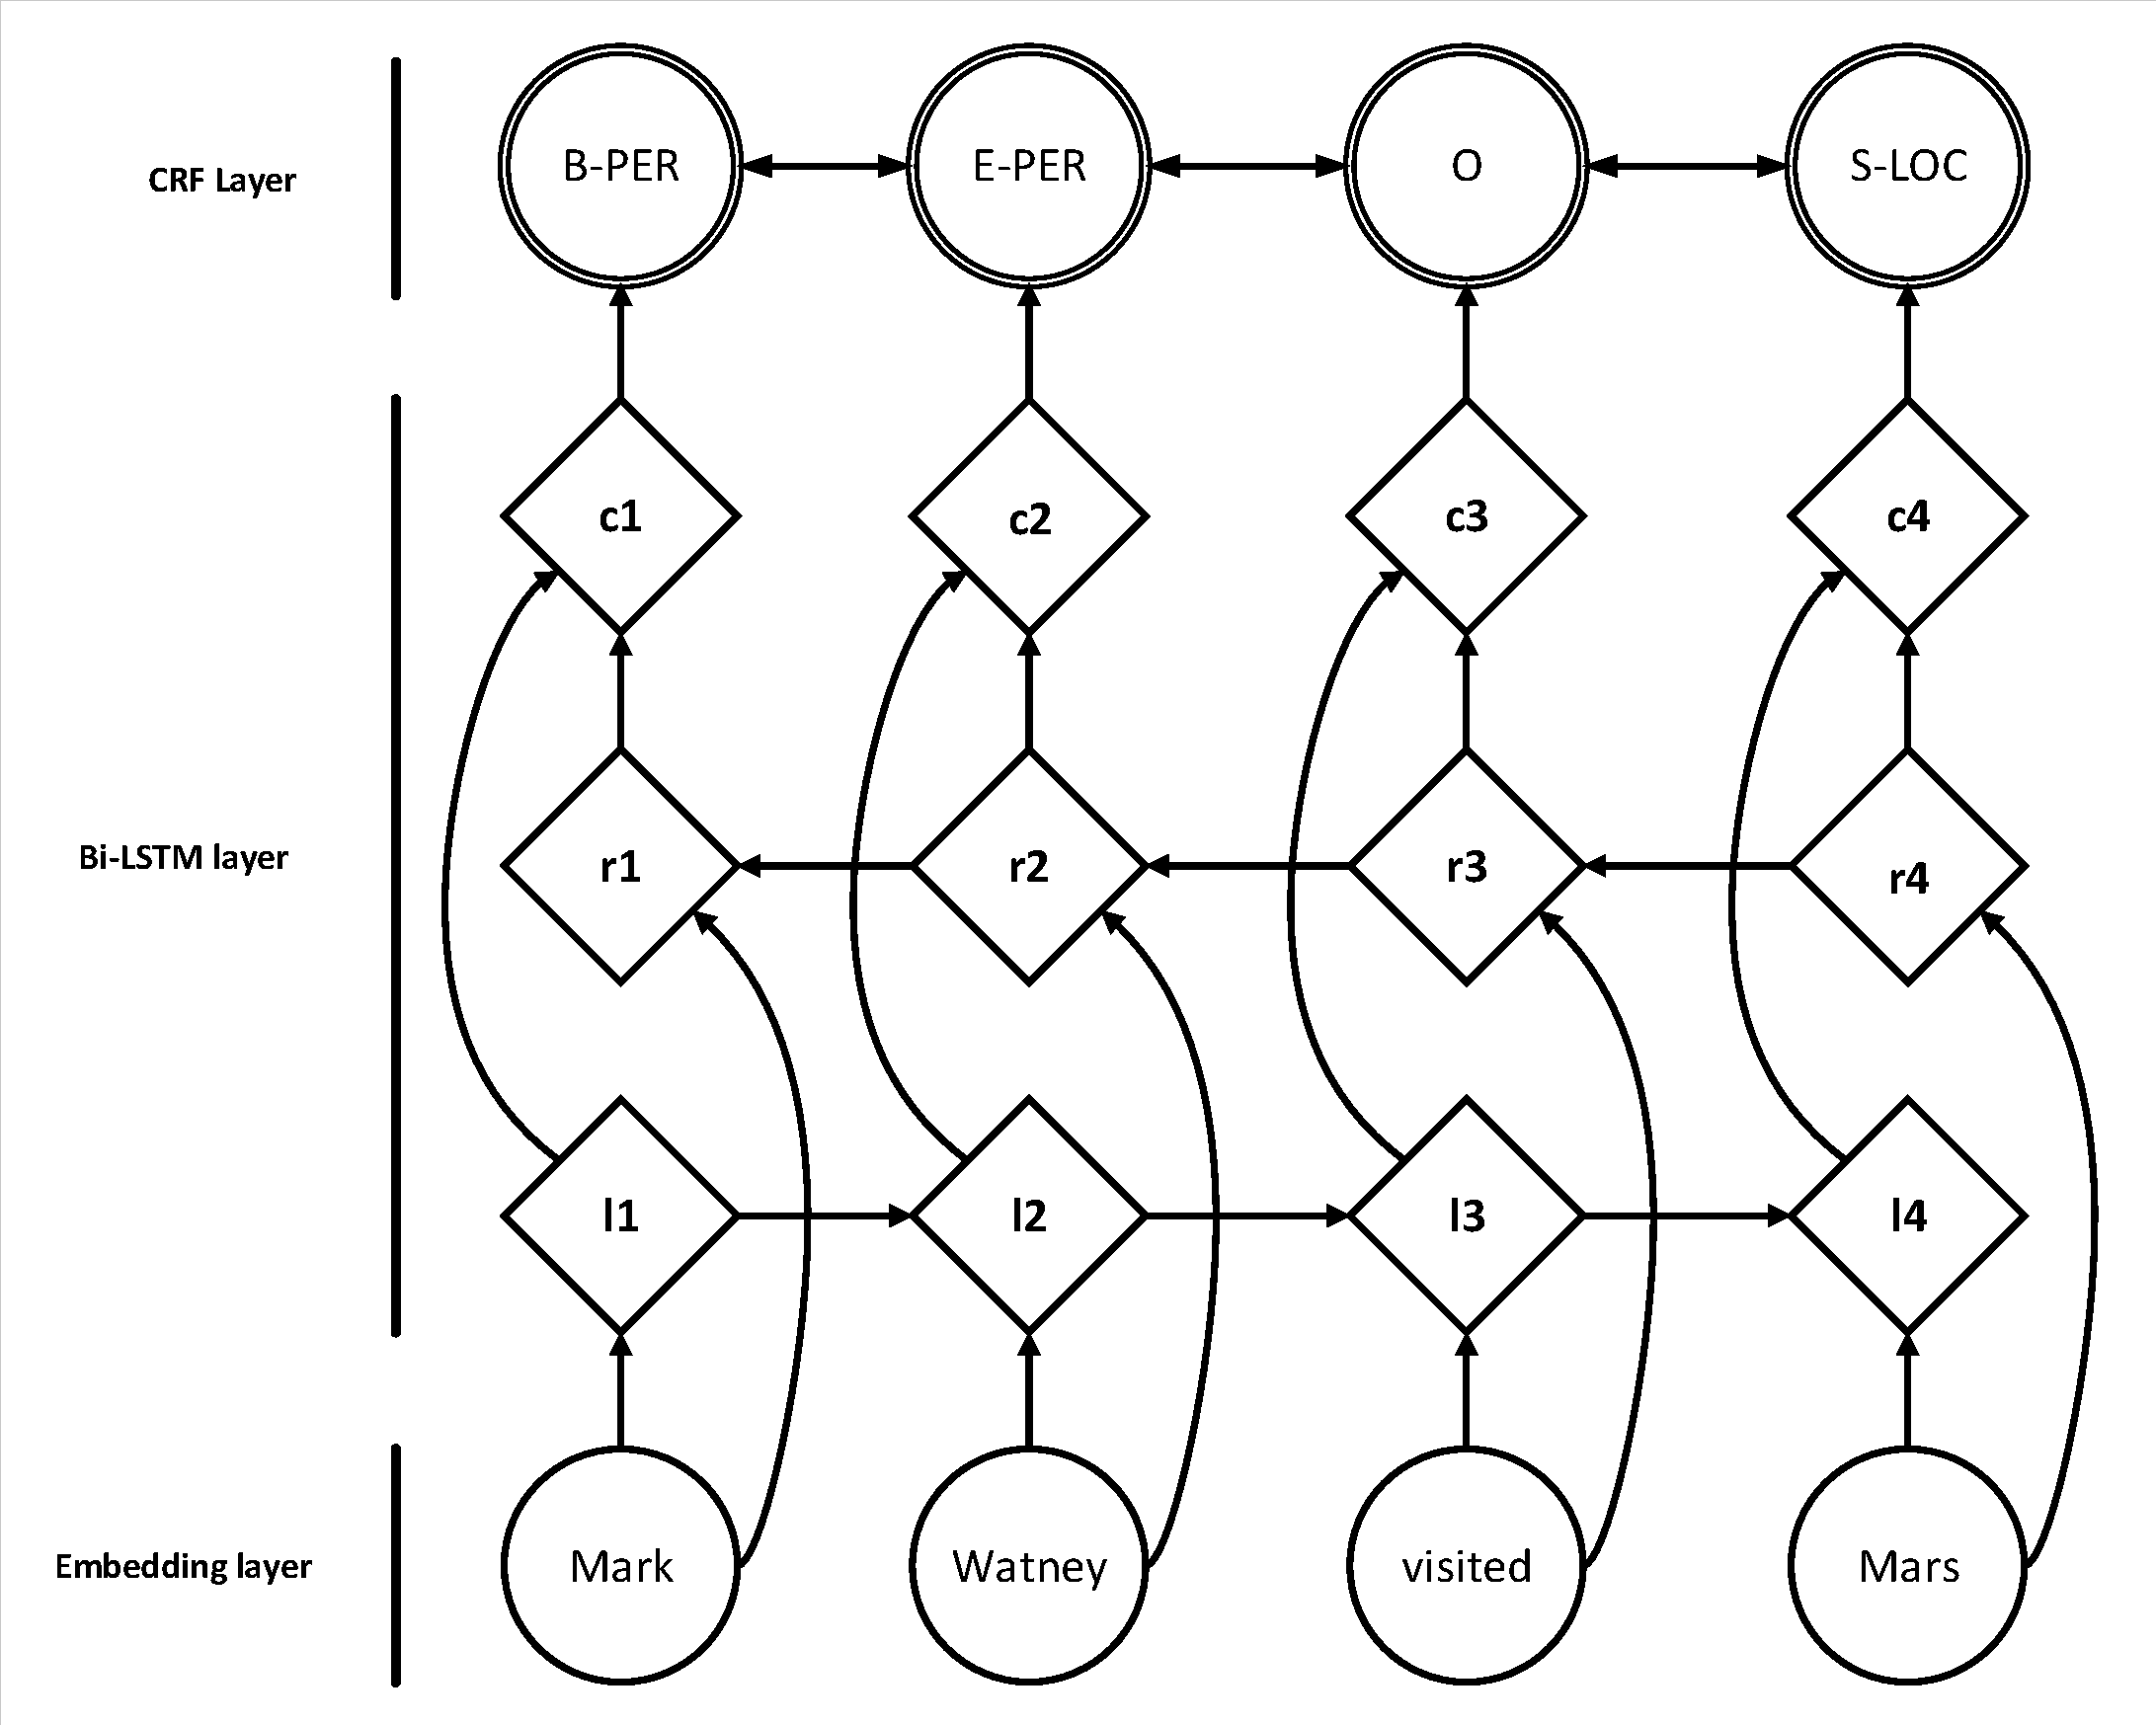
\includegraphics[width=0.8\textwidth, trim=2 2 2 2, clip]{resources/3/blstmcrf.pdf}
	\caption{Arsitektur LSTM dua arah dengan CRF \parencite{lample2016neural}}
	\label{fig:blstmcrf}
\end{figure}

\subsection{LSTM Dua Arah dan CNN}

Gambar \ref{fig:blstmcnn} menunjukkan arsitektur LSTM dua arah dengan CNN \parencite{chiu2015named}. Arsitektur ini melibatkan CNN sebagai eksraksi fitur sebuah kata dalam kalimat. Hasil dari ekstraksi tersebut menjadi masukan untuk kedua LSTM yang berbeda arah untuk melakukan latihan \textit{sequence labeling}.

\begin{figure}[H]
	\centering
	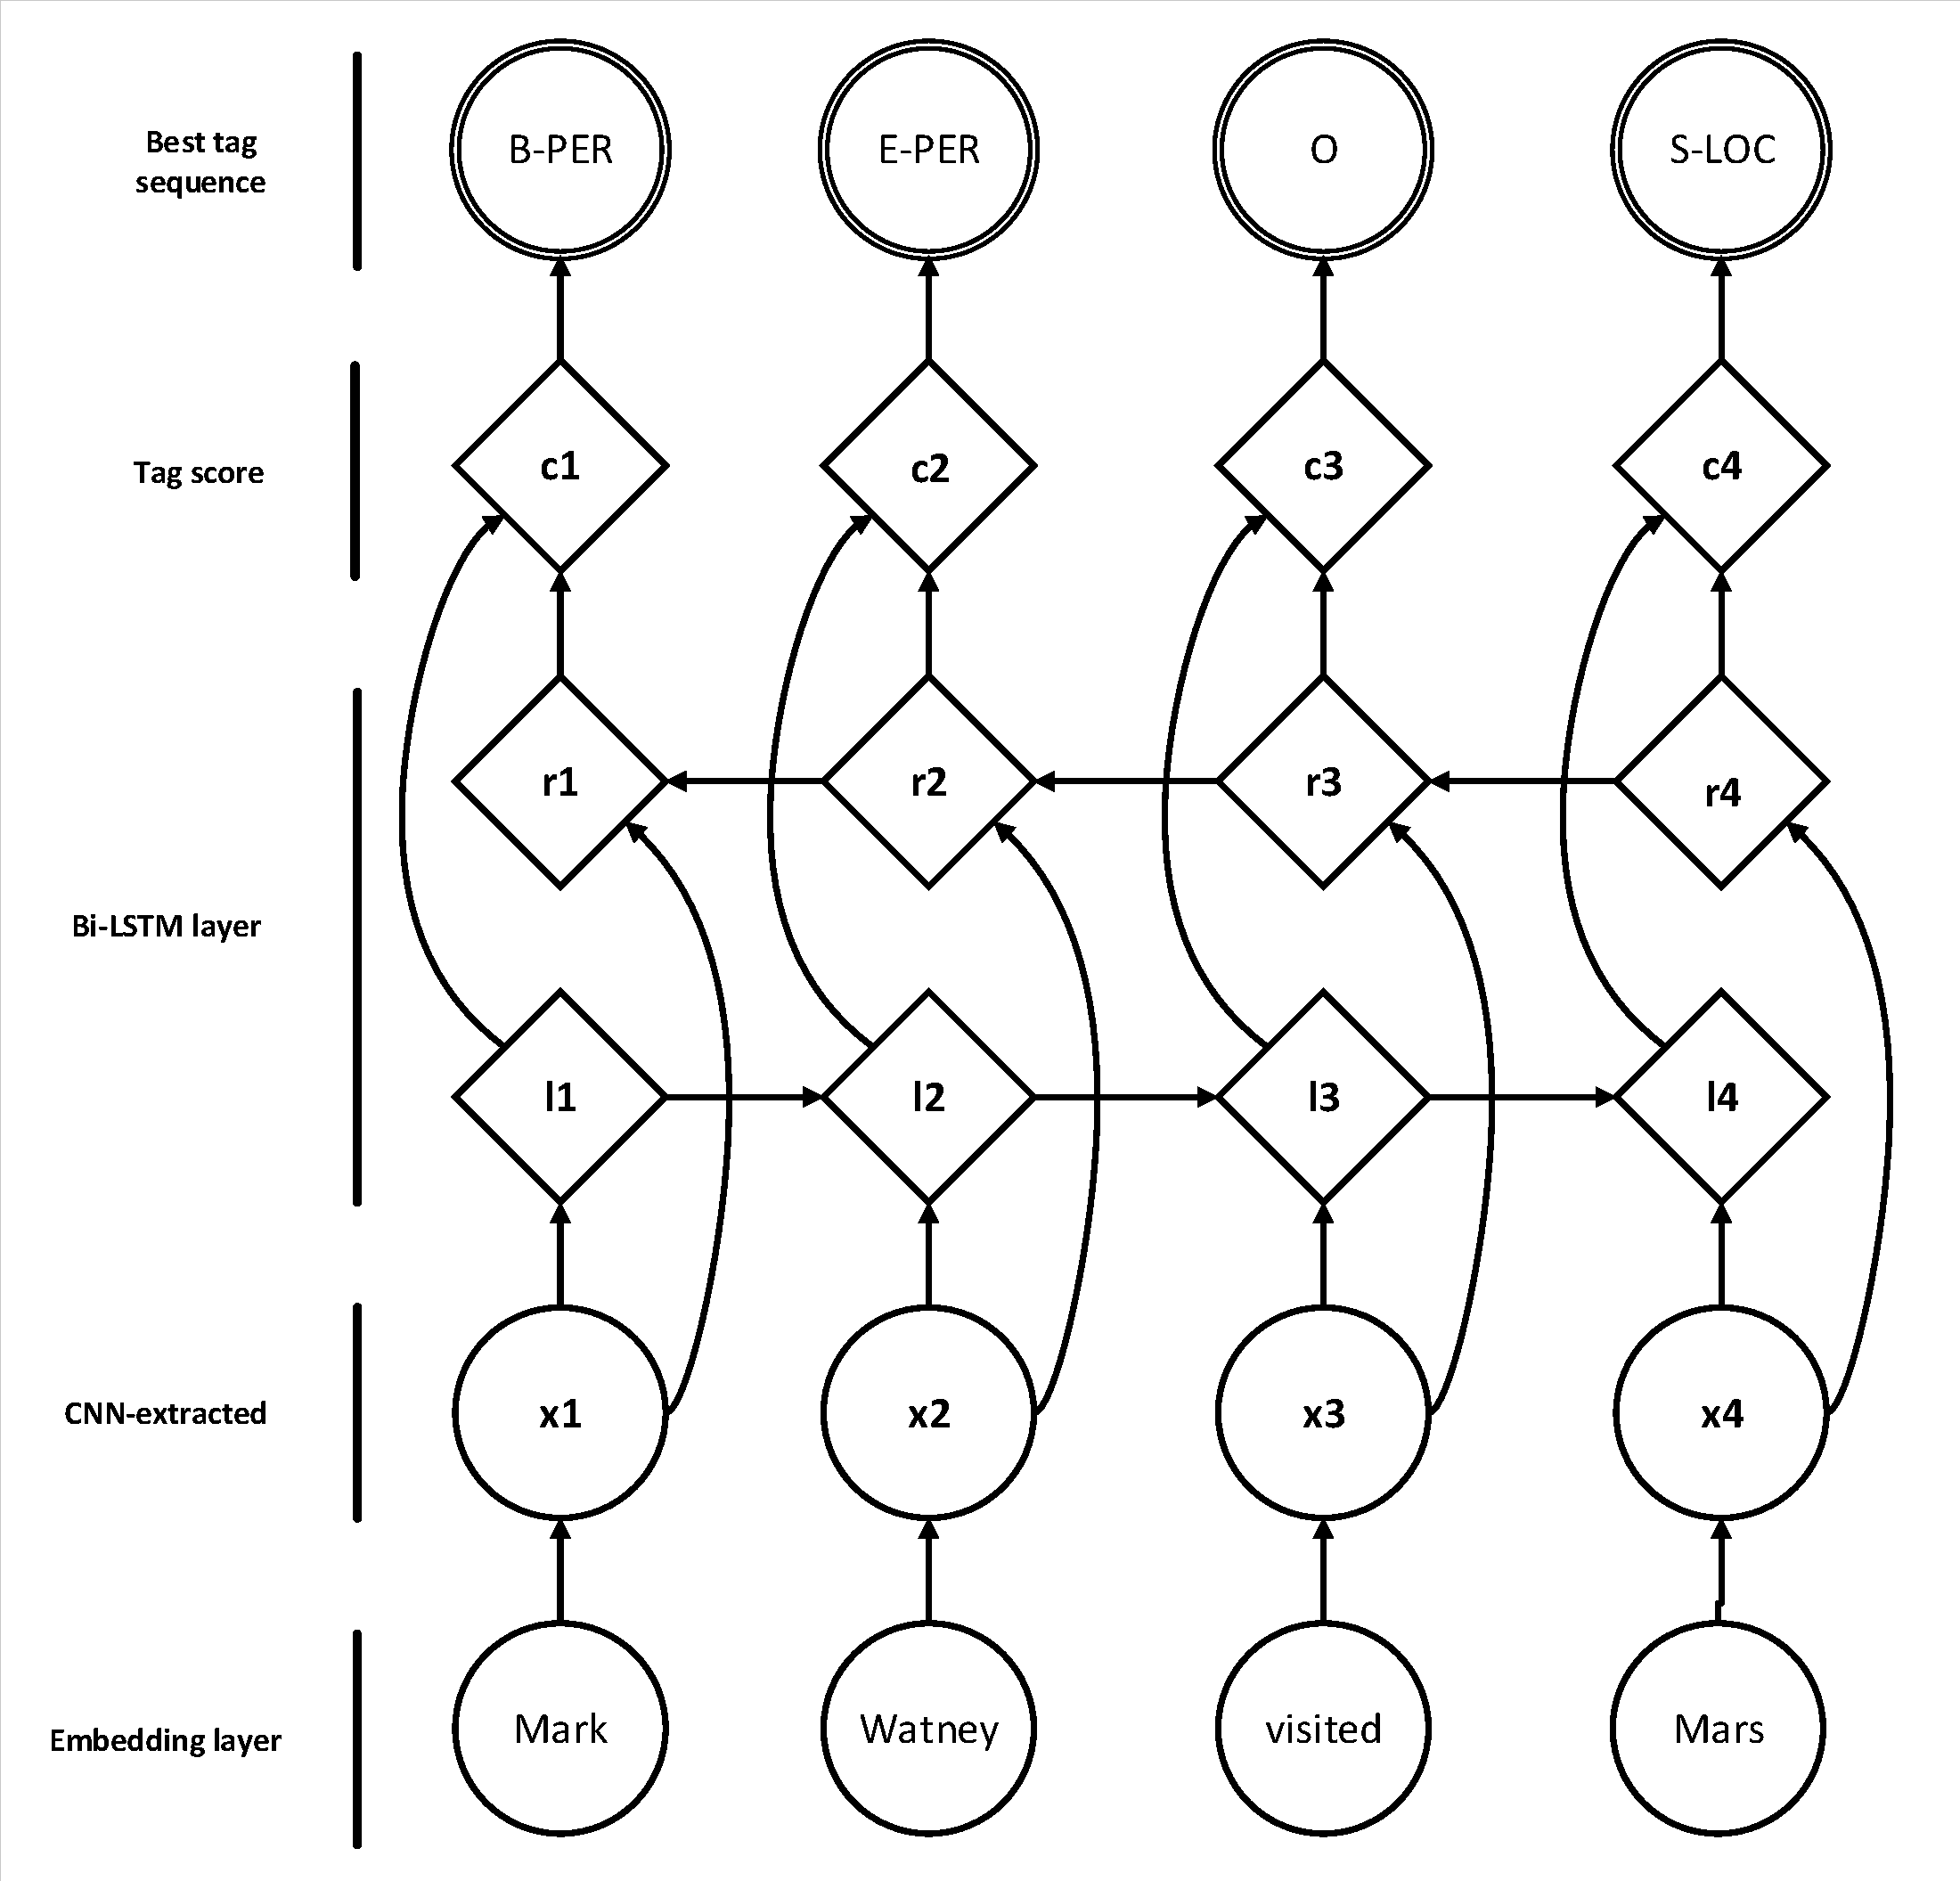
\includegraphics[width=0.8\textwidth, trim=2 2 2 2, clip]{resources/3/blstmcnn.pdf}
	\caption{Arsitektur LSTM dua arah dengan CNN \parencite{chiu2015named}}
	\label{fig:blstmcnn}
\end{figure}

\section{Rancangan Sistem}

\subsection{Rancangan Latihan Klasifikasi}

Rancangan sistem untuk tahap latihan klasifikasi disajikan dalam bagan pada Gambar \ref{fig:design_training} berikut. Proses-proses yang harus dilewati dalam tahap latihan klasifikasi dapat dijelaskan sebagai berikut:

\begin{enumerate}
	\item sistem akan memuat \textit{file} JSON yang berisi data latihan yang digunakan untuk membangun NLU,
	\item sistem mengambil data latihan tersebut lalu mengubahnya menjadi sekumpulan obyek SentenceData,
	\item sistem mengambil informasi maksud kalimat yang telah didefinisikan di dalam data latihan dan menyimpan sekumpulan maksud kalimat,
	\item sistem memecahkan sebuah kalimat menjadi sekumpulan \textit{token} kata,
	\item sistem mengekstraksi entitas yang telah didefinisikan di dalam data latihan dan mengumpulkan semua entitas yang terekstrasi,
	\item sistem menciptakan tas kata-kata dengan menggunakan metode \textit{one-hot encoding},
	\item sekumpulan maksud kalimat dan tas kata-kata digunakan sebagai masukan untuk latihan model NLU, menghasilkan model klasifikasi, dan,
	\item model klasifikasi disimpan ke dalam direktori sistem untuk digunakan pada tahap klasifikasi teks.
\end{enumerate}

\begin{figure}[H]
	\centering
	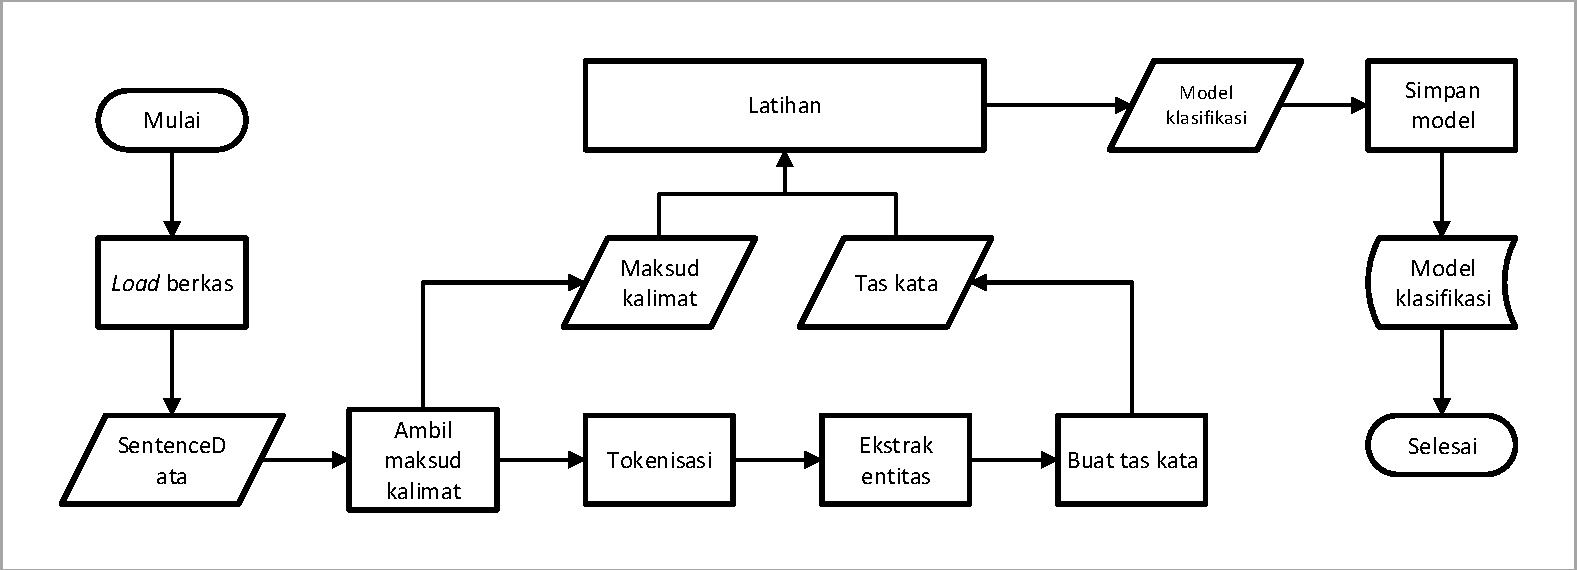
\includegraphics[width=\textwidth, trim=2 2 2 2, clip]{resources/3/design_training.pdf}
	\caption{Bagan rancangan sistem tahap latihan klasifikasi}
	\label{fig:design_training}
\end{figure}

\subsection{Rancangan Klasifikasi Teks}

Rancangan sistem untuk tahap klasifikasi teks disajikan dalam bagan pada Gambar \ref{fig:design_classification}. Proses-proses yang harus dilewati dalam tahap klasifikasi teks dapat dijelaskan sebagai berikut:

\begin{enumerate}
	\item sistem menerima masukan teks dari \textit{speech recognition} yang dimasukkan oleh suara pengguna,
	\item sistem memecahkan teks menjadi sekumpulan \textit{token},
	\item sistem mengenali entitas yang berada di dalam teks, kemudian mengekstraksi entitas tersebut,
	\item sistem menciptakan tas kata-kata untuk teks masukan,
	\item sistem melakukan prediksi maksud kalimat dari masukan tas kata-kata menggunakan model klasifikasi yang dihasilkan pada tahap latihan klasifikasi,
	\item maksud kalimat yang telah dihasilkan, bersama dengan kumpulan entitas hasil ekstrasi, menjadi masukan untuk memenggil aksi sistem, dan,
	\item sistem melakukan aksi kepada pengguna sebagai tanggapan dari masukan teks dari sistem ASR.
\end{enumerate}

\begin{figure}[H]
	\centering
	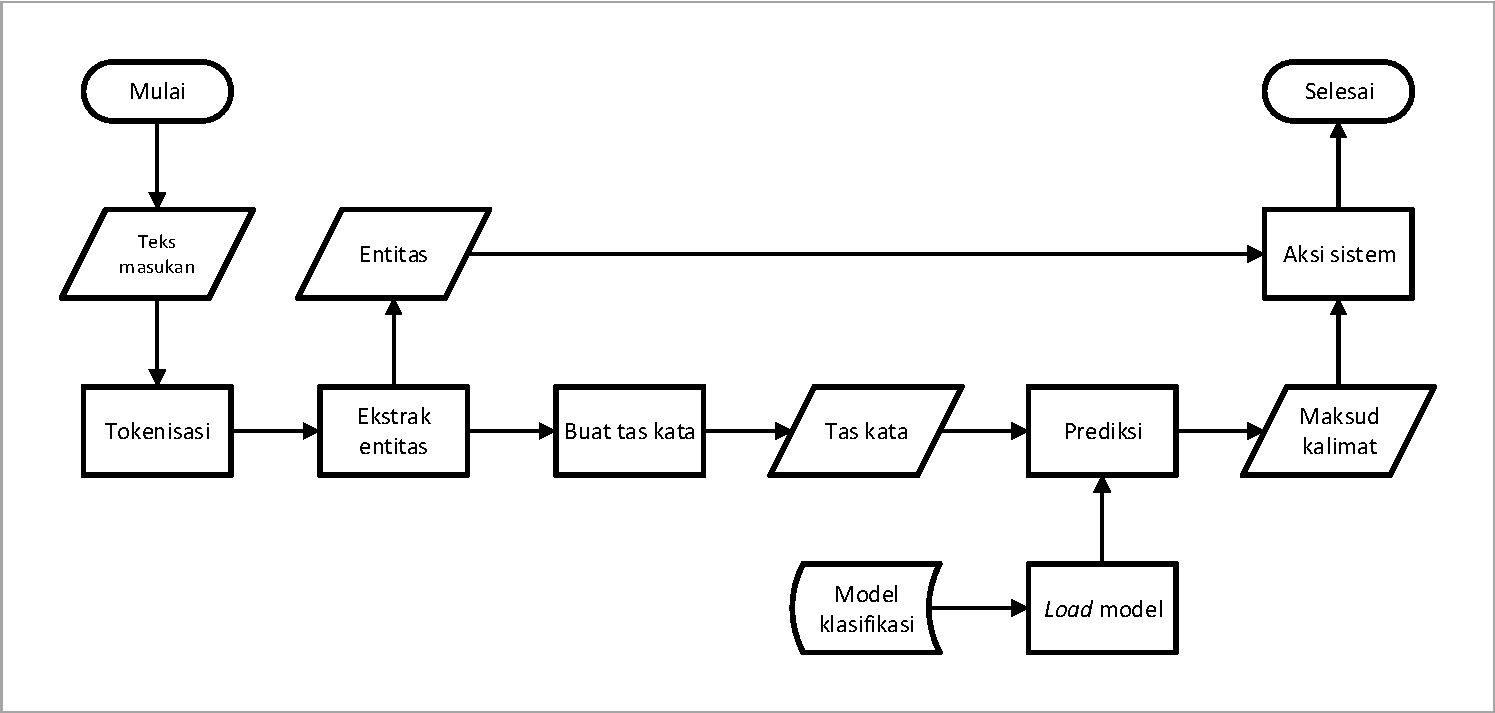
\includegraphics[width=\textwidth, trim=2 2 2 2, clip]{resources/3/design_classification.pdf}
	\caption{Bagan rancangan sistem tahap klasifikasi teks}
	\label{fig:design_classification}
\end{figure}

\section{Alat-Alat yang Digunakan untuk Pengembangan}

Pengembangan sistem ini dilakukan di dalam lingkungan sistem operasi Windows 10. Pengembangan sistem menggunakan bahasa Python versi 3.6.6 dalam lingkungan Anaconda, dan \textit{library} yang digunakan adalah sebagai berikut:

\begin{enumerate}
    \item Keras, dengan versi 2.1.6
    \item scikit-learn, dengan versi 0.19.1
    \item sklearn-crfsuite, dengan versi 0.3.6
\end{enumerate}